\documentclass[12pt, oneside]{article} 
\usepackage[a4paper]{geometry}              
\usepackage{graphicx}
\usepackage{amsmath}
\usepackage{amssymb}
\usepackage[table]{xcolor}

%SetFonts
\usepackage[T1]{fontenc}
\usepackage[bitstream-charter]{mathdesign}
%SetFonts

%define example environment 
\newcounter{examplecounter}
\newenvironment{example}%
{%
\small\begin{quote}%
\refstepcounter{examplecounter}%
\textbf{Example \arabic{examplecounter}}%
\quad%
}%
{%\schluss%
\end{quote}%
}

%define remark environment 
\newcounter{remarkcounter}
\newenvironment{remark}%
{%
\small\begin{quote}%
\refstepcounter{remarkcounter}%
\textbf{Remark \arabic{remarkcounter}}%
\quad%
}%
{%\schluss%
\end{quote}%
}

%define remark environment 
\newcounter{questioncounter}
\newenvironment{question}%
{%
\small\begin{quote}%
\refstepcounter{questioncounter}%
\textbf{Question \arabic{questioncounter}}%
\quad%
}%
{%\schluss%
\end{quote}%
}


%define important environment
\newenvironment{important}{\begin{quote}%
\textbf{Important:}%
\quad
}{%
\end{quote}%
}

\newcommand{\qed}{\nobreak \ifvmode \relax \else
      \ifdim\lastskip<1.5em \hskip-\lastskip
      \hskip1.5em plus0em minus0.5em \fi \nobreak
      \vrule height0.5em width0.5em depth0.25em\fi}

\newtheorem{theorem}{Theorem}[section]
\newtheorem{corollary}{Corollary}[section]
\newtheorem{lemma}[theorem]{Lemma}
\newtheorem{proposition}[theorem]{Proposition}
\newtheorem{definition}{Definition}
\newenvironment{proof}[1][Proof]{\begin{trivlist}
\item[\hskip \labelsep {\bfseries #1}]}{\end{trivlist}}

\newcommand{\R}{\mathbb{R}}
\newcommand{\C}{\mathbb{C}}
\newcommand{\E}{\mathbb{E}}
\newcommand{\fol}{\mathcal{F}}
\newcommand{\one}{\mathbb{1}}
\newcommand{\rank}{\text{rank}}
\newcommand{\detp}{{\det}_+}

\usepackage{lettrine}

\begin{document}
\noindent{\Huge \textbf\textsf{{Completing correlation matrices}}}

\noindent \textit{by Horst K�hler, Thomas Streuer, Olaf Dreyer}

\vspace{.5cm}

\section{Introduction}

\section{The completion criterium}
Given a correlation matrix with unknown coefficients what is the right way to complete it? To motivate the answer we need to introduce some notation. Let 
\begin{equation}
	X = ( x_1, \ldots, x_k )^T\in \R^k
\end{equation}
be a $k$ dimensional random variable with a density function given by a $k$ dimensional normal distribution
\begin{align}
	f(X) & = N_k[\mu, H_X]( X ) \\
	& = (2\pi)^{-k/2}\det(H_X)^{-1/2}\exp\left(-\frac{1}{2}(X -\mu)^T H_X^{-1} (X-\mu)\right),
\end{align}
with mean $\mu$ and covariance matrix $H_X$. A crucial property of the normal distribution is that if we condition on some of the $x_i$, $i=1, \dots, k$, we again obtain a normal distribution. Let us assume that we want to condition on the last $l$ components of $X$:
\begin{equation}
	Z = (x_{k-l+1}, \ldots, x_k)^T \in \R^l.
\end{equation}
We partition the matrix $H$ in a way that reflects this partition of $X$:
\begin{equation}
	H_X = \begin{pmatrix}
		A & B \\
		B^T & C
	\end{pmatrix},
\end{equation}
with $A\in M_{k-l}$, $C\in M_l$, and $B\in M_{k-l,l}$. Let $\bar X$ be the first $k-l$ components of $X$:
\begin{equation}
	\bar X = (x_1, \ldots, x_{k-l})^T\in \R^{k-l}
\end{equation}
If we assume that $X$ has zero mean (i.e. $\mu=0$), the density function for $X$ conditioned on $Z$ is then given by
\begin{equation}
	f(X \vert Z ) = N_{k-l}[BC^{-1}Z, H_X/C ](\bar X),
\end{equation}
(see \cite[chapter 8]{rao} and \cite{cottle}) where $H_X/C$ is the Schur complement of $C$ in $H_X$:
\begin{equation}\label{eqn.hxc}
	H_X/C = A - B C^{-1}B^T
\end{equation}
(Emilie Haynsworth introduced the name and highlighted its usefulness in \cite{hayns}. Schur originally made use of it in \cite{schur}. For an overview of the properties of the Schur complement see \cite{horn}.) We see that we again obtain a normal distribution. We will meet the Schur complement again soon.

Now let us look at a second set of random variables 
\begin{equation}
	Y = (x_{k-l+1}, \ldots, x_k, x_{k+1}, \ldots, x_n)^T \in \R^{n-k},
\end{equation}
that has an overlap $Z$ with the random variables $X$. Let the density function for $Y$ be given by
\begin{equation}
	f(Y) = N_{n-k}[0,H_Y] ( Y),
\end{equation}
with
\begin{equation}
	H_Y = \begin{pmatrix}
		C & D \\
		D^T & E
	\end{pmatrix}.
\end{equation}
Note that the submatrix $C$ is shared with $H_X$. In our context the matrix $C$ might have been obtained by a previous calibration of a model that is part of both $X$ and $Y$. If we were to condition on $Z$ we would find
\begin{equation}
	f(Y\vert Z) = N_{n-k-l}[ D^T C^{-1}Z,H_Y/C](\bar Y), 
\end{equation}
with
\begin{equation}\label{eqn.hyc}
	H_Y/C = E - D^TC^{-1}D
\end{equation}
and $\bar Y$ is the part of $Y$ that is not $Z$. If we now want to describe $X$ and $Y$ together we are looking at the matrix
\begin{equation}
	H = \begin{pmatrix}
		A & B & W \\
		B^T & C & D \\
		W^T & D^T & E
	\end{pmatrix},
\end{equation}
with a yet to be determined matrix $W\in M_{k-l,n-l}$. Because $X$ and $Y$ share the random variables in $Z$ we can not make them independent. The next best thing that we can do is to demand that if we fix $Z$ the remaining parts of $X$ and $Y$ are independent. The combined density for $X$ and $Y$ when we condition on $Z$ is given by
\begin{equation}
	f( X,Y\vert Z) = N_{n-l}[ (B^T,D)^TC^{-1}Z, H/C](\bar X, \bar Y),
\end{equation}
with
\begin{align}
	H/C & = \begin{pmatrix}
		A - B C^{-1}B^T & W - B C^{-1} D \\
		W^T - D^TC^{-1}B^T & E - D^TC^{-1}D
	\end{pmatrix}\\
  & = \begin{pmatrix}
		H_X/C & W - B C^{-1} D \\
		W^T - D^TC^{-1}B^T & H_Y/C
	\end{pmatrix}.
\end{align}
We see that if we set
\begin{equation}\label{eqn.choice}
	W = BC^{-1}D
\end{equation}
the above matrix becomes block diagonal and the conditional densities obey
\begin{equation}\label{eqn.independent}
	f(X,Y\vert Z ) = f(X\vert Z)f(Y\vert Z)
\end{equation}
because the blocks in the diagonal are $H_X/C$ and $H_Y/C$ from equations (\ref{eqn.hxc}) and (\ref{eqn.hyc}). Given that $Z$ is part of both $X$ and $Y$ this is as much independence as we can ask for. The way to choose the matrix $W$ and complete $H$ is to demand that $X$ and $Y$, when conditioned on their shared part $Z$, are independent.

This choice of $W$ can be characterized in two more ways (see \cite{smith} and \cite{ksd}). Banachiewicz showed that the inverse of a matrix can be expressed using the Schur complement. Since the Schur complement $H/C$ is block diagonal the inverse of $H$ is given by
\begin{equation}
	H^{-1} = \begin{pmatrix}
		(H_X/C)^{-1} & -(H_X/C)^{-1} B C^{-1} & 0 \\
		- C^{-1} B^T (H_X/C)^{-1} & \Xi & - C^{-1} D (H_Y/C)^{-1} \\
		0 & - (H_Y/C)^{-1} D^T C^{-1} & (H_Y/C)^{-1} 
	\end{pmatrix},
\end{equation}
with
\begin{equation}
\Xi = C^{-1} + C^{-1} B^T (H_X/C)^{-1} B C^{-1} + C^{-1} D (H_Y/C)^{-1} D^T C^{-1}.
\end{equation}
We see that $H^{-1}$ has zeroes in the places where $W$ sits in $H$. The $W$ from equation (\ref{eqn.choice}) is the unique choice with that property.  

When looking at the determinant of $H$ we find another characterization of $W$. Using the Schur complement again, we find
\begin{align}
	\det H & = \det C \; \det H/C \\
	& \le \det C \; \det H_X/C \; \det H_Y/C,\label{eqn.fischer}
\end{align}
where we have equality in equation (\ref{eqn.fischer}) if and only if the off-diagonal blocks vanish, i.e. if and only if $W$ is given by equation (\ref{eqn.choice}). This choice of $W$ is the unique choice that maximizes the determinant of $H$.

The entropy $S$ of the normal distribution $N_n[\mu,H]$ is given by
\begin{equation}
	S = \frac{1}{2}\log \det H + \text{\ const.}
\end{equation} 
Because we are maximizing the determinant of $H$ we are also maximizing the entropy $S$ of the distribution described by $H$. The $H$ chosen by the $W$ from equation (\ref{eqn.choice}) is the one that puts the fewest constraints on the distribution of $X$ and $Y$. 

\section{The completion procedure}
In the last section we have completed the matrix $H$ in the very simple case where there are two known matrices $H_X$ and $H_Y$ with just one shared part $C$. The general case is usually more complicated. Building on the result in \cite{grone} Smith \cite{smith} (see also \cite{ksd} for a more general treatment of the semidefinite case) showed how to solve the general problem by reducing it to a repeated application of the result from the previous section. We will discuss the required steps in this section by looking at a particular example: the cross currency model.

Our model will consist of two interest rate models; one for the base currency $E$ and one the foreign currency $A$. These two currencies are linked by an exchange rate $X$. We will model the two interest rates and the exchange rate with stochastic volatility models so that we have a total of six stochastic variables:
\begin{equation}\label{eqn.stochvar}
	E, \nu_E, A, \nu_A, X, \nu_X
\end{equation}
We will denote the corresponding correlation coefficients by 
\begin{equation}
	(a,b),
\end{equation}
where $a$ and $b$ are one of the stochastic variables from equation (\ref{eqn.stochvar}). In total there are 15 different correlation coefficients in the correlation matrix $H$ of our model. We assume that the coefficients 
\begin{equation}
	(E,\nu_E)\text{\ and\ }(A,\nu_A)
\end{equation}
have already been determined in separate calibrations of the interest rate models. That leaves us with 13 free coefficients in $H$. This number of coefficients is too large for a stable calibration. Instead we will only calibrate the coefficients
\begin{equation}
	(E,A), (E,X), (A,X),(X,\nu_X),
\end{equation}
and determine the remaining nine coefficients using the completion procedure described here (see figure \ref{fig.xccymodel}).

\begin{figure}[hbt]
  \begin{center}
  	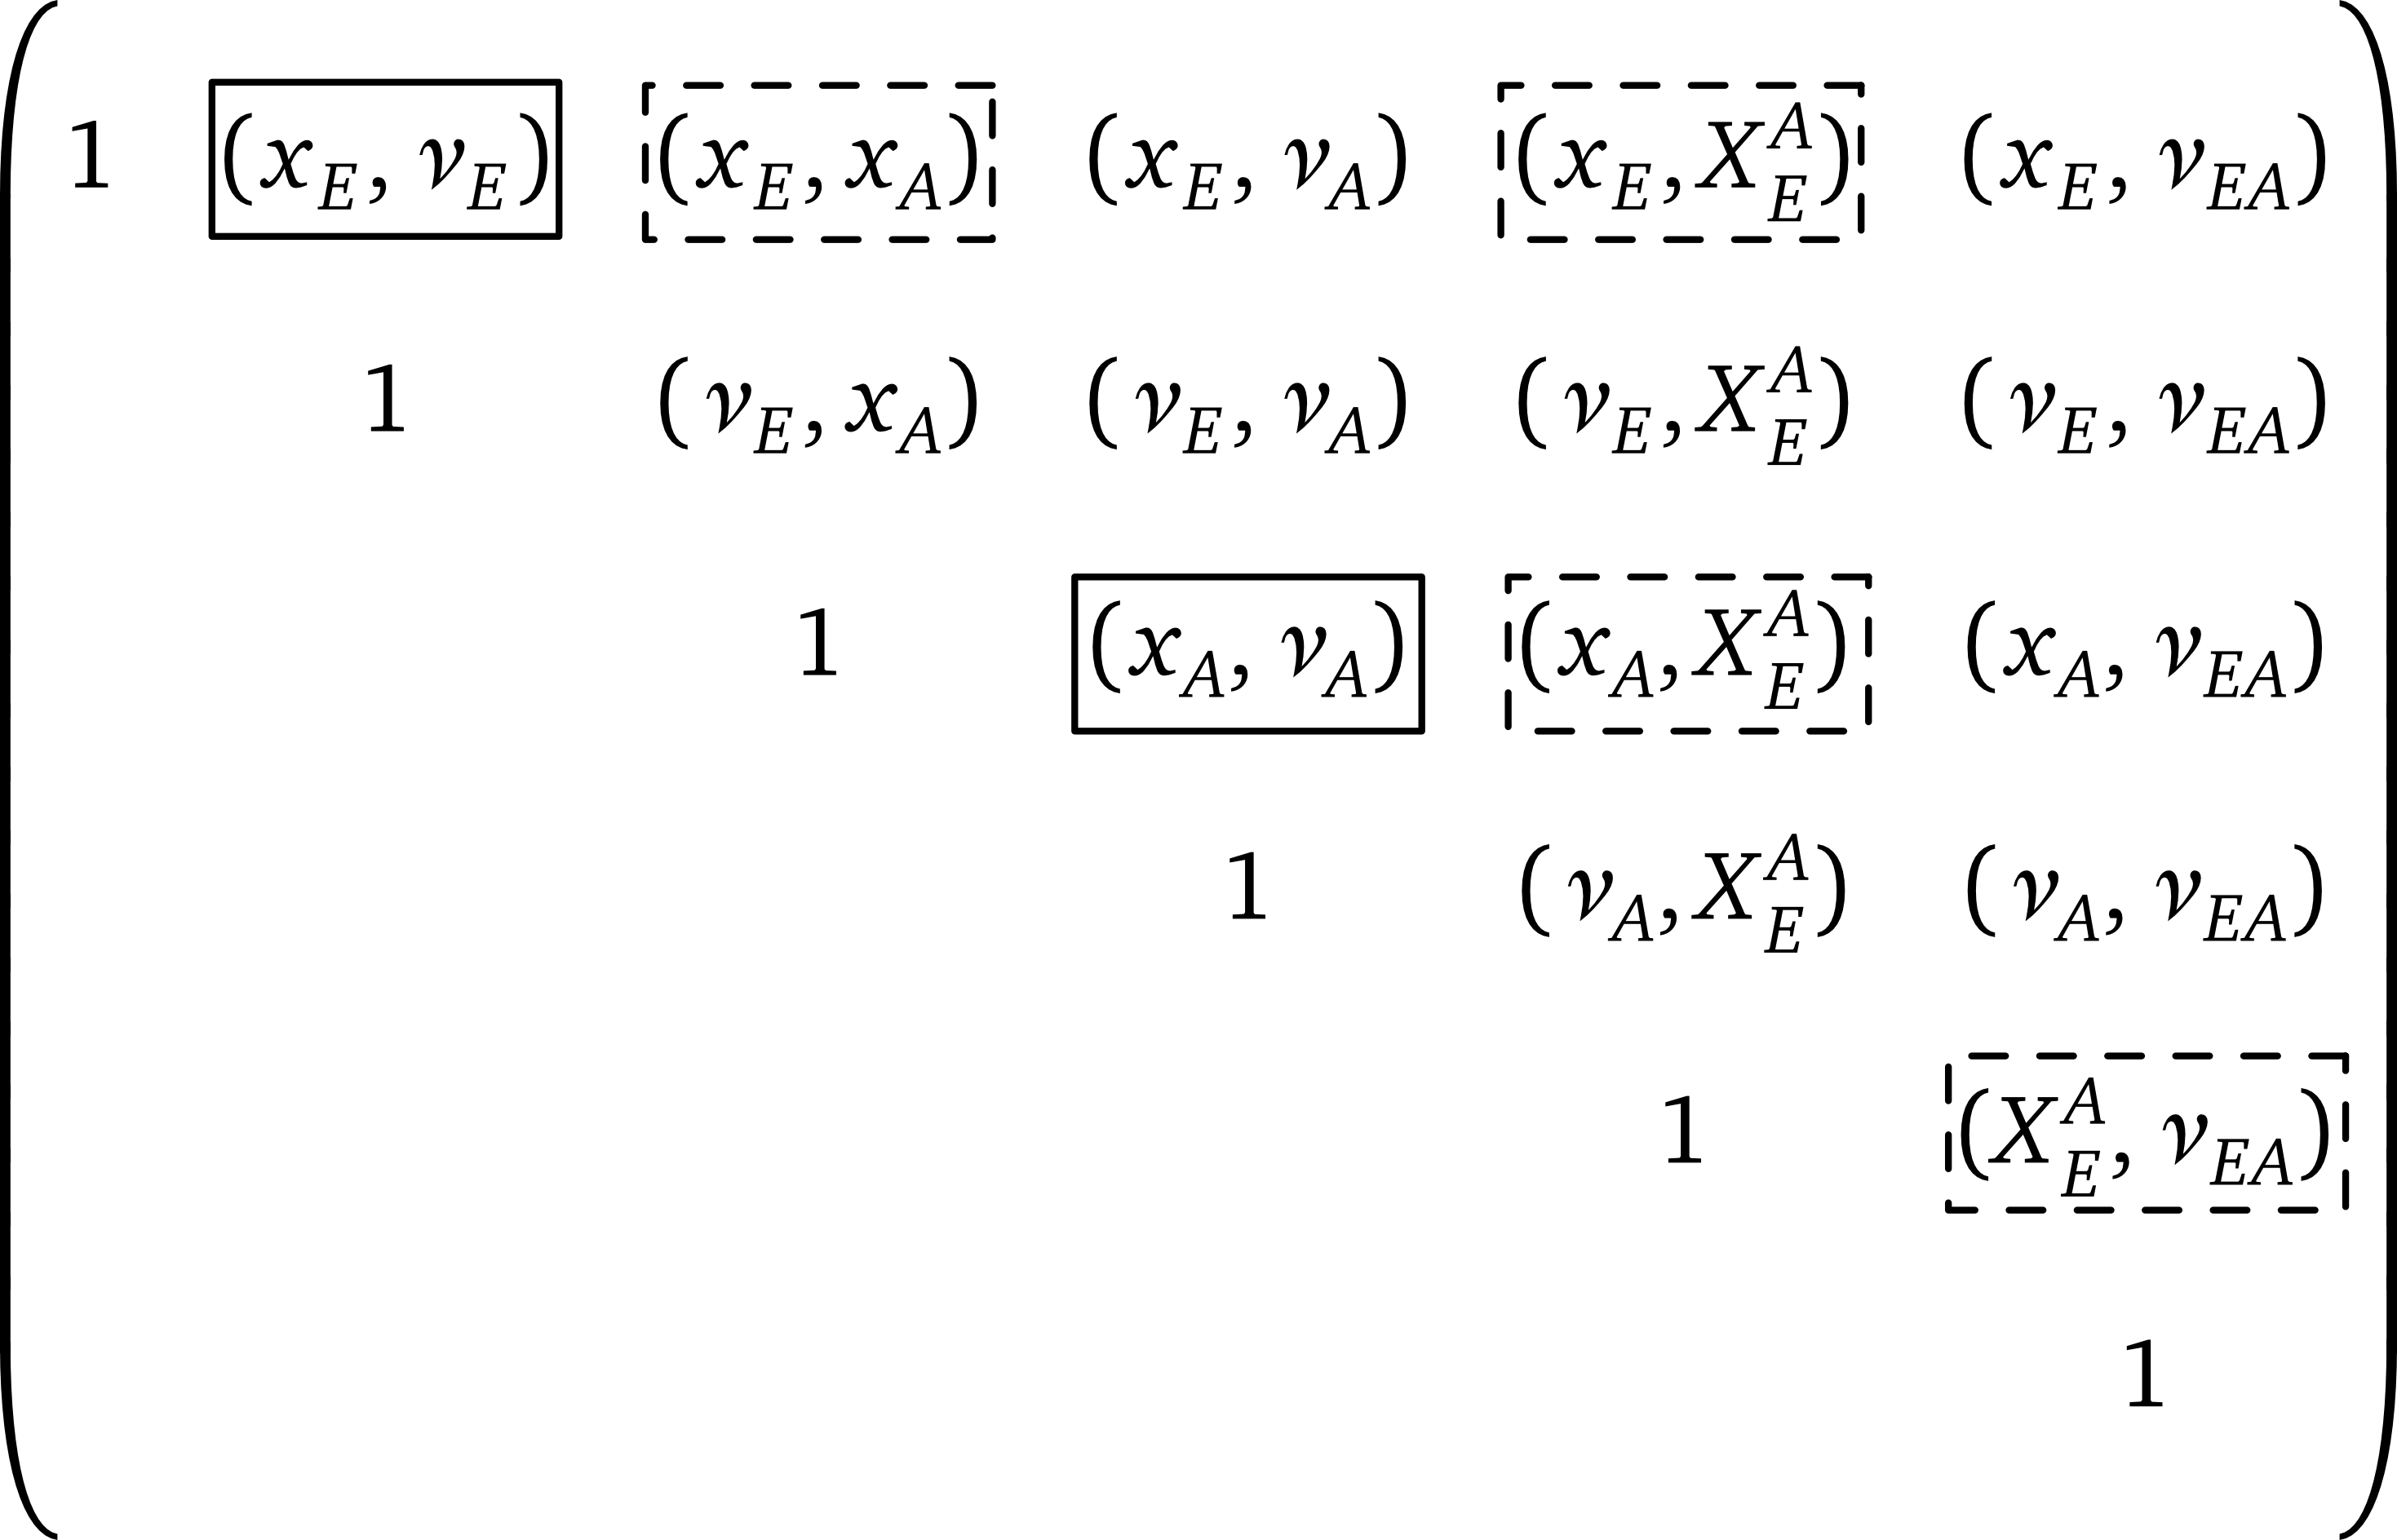
\includegraphics[width=10cm]{img/xccymodel.png}
  \end{center}
  \caption{The correlation matrix for the cross currency model. The coefficients $(E, \nu_E)$ and $(A, \nu_A)$ (the boxes with the dashed lines) are determined in separate interest rate calibrations. The coefficients $(E, X)$, $(E, A)$, $(A, X)$, and $(X, \nu_X)$ (the boxes with the solid lines) will be determined in the cross currency calibration itself. The remaining coefficients are the result of the completion procedure.}\label{fig.xccymodel}
\end{figure}

The first step to complete the matrix $H$ is to determine the graph $\gamma$ corresponding to $H$. The vertices of the graph are given by the row (or column) indices of $H$. In our case these are identified with the stochastic variables in equation (\ref{eqn.stochvar}). We then obtain the graph for $H$ by connecting the vertices for which we have coefficients. In our example we obtain the graph in figure \ref{fig.fxCalibrationGraph}.

\begin{figure}[hbt]
  \begin{center}
  	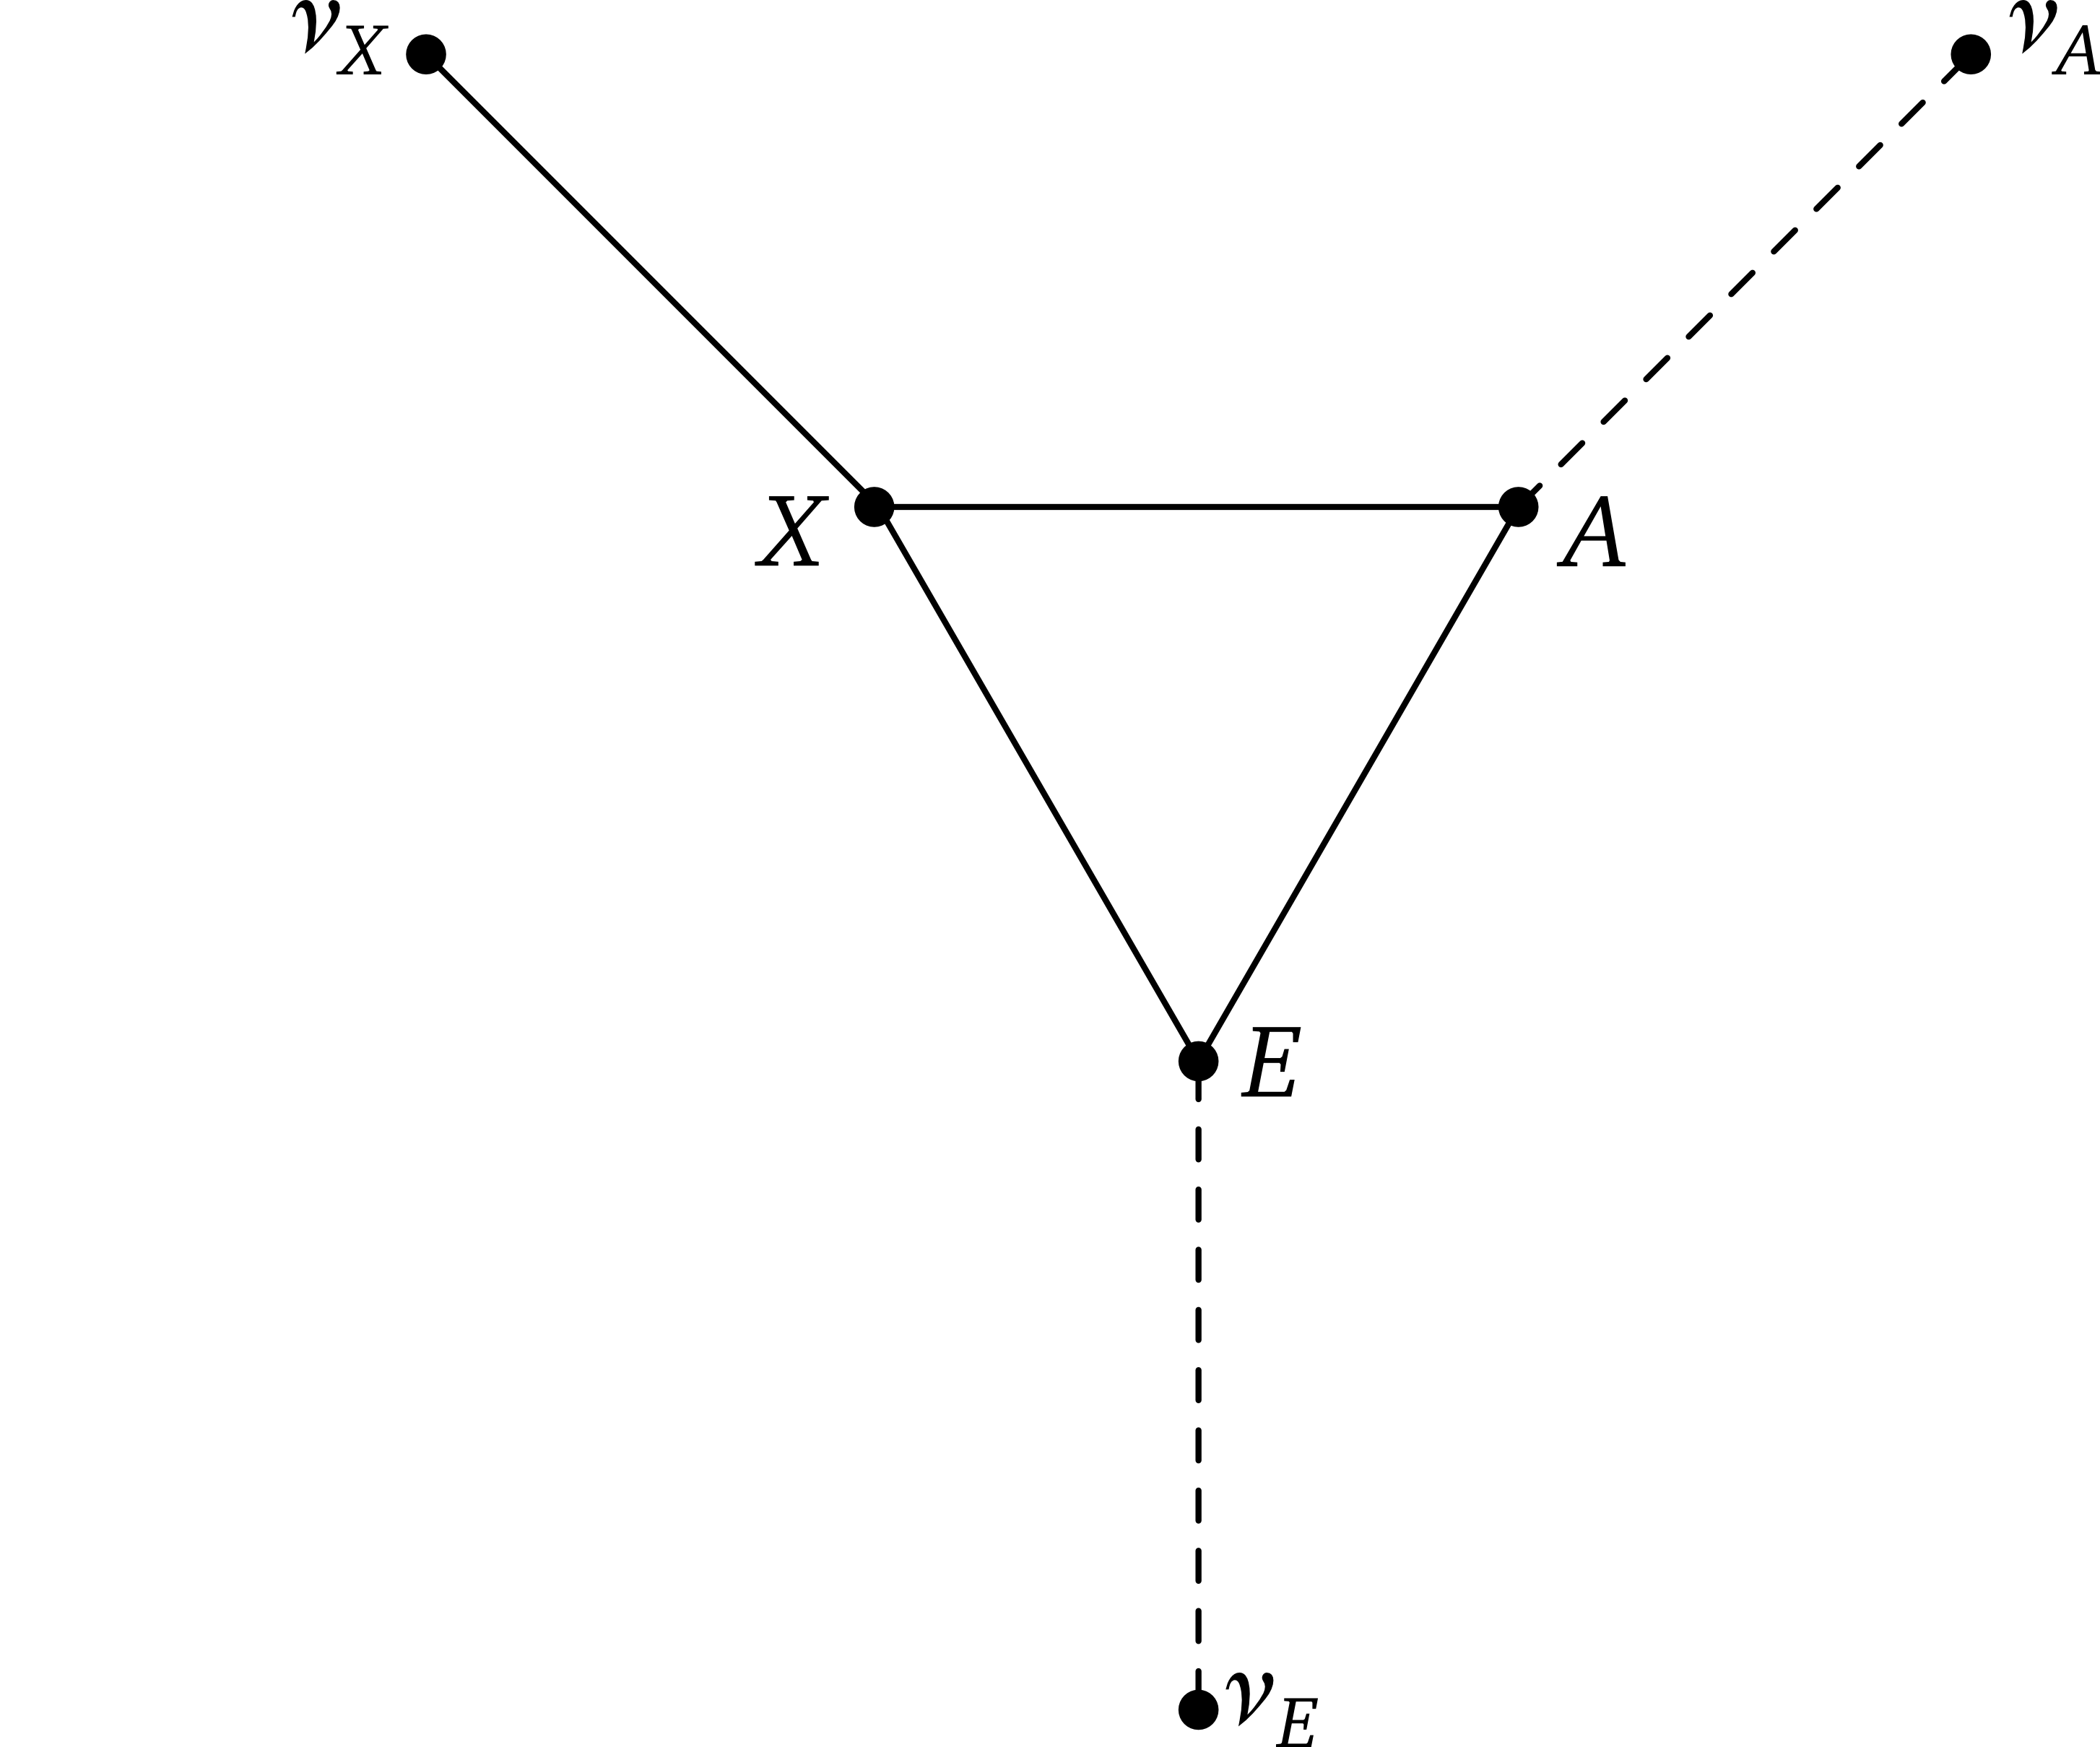
\includegraphics[width=10cm]{img/fxCalibrationGraph.png}
  \end{center}
  \caption{The initial graph $\gamma$ for the cross currency calibration. The coefficients $(E,\nu_E)$ and $(A,\nu_A)$ (dashed edges) are determined in separate interest rate calibrations. The other edges are determined in the cross currency calibration itself.}\label{fig.fxCalibrationGraph}
\end{figure}

Now that we have the graph we need to determine if the graph is chordal. A graph is chordal if every loop of length four or more has a chord (i.e. an edge connecting two non-consecutive vertices in the loop; see e.g. \cite{golumbic}). In our example this is easy to check. The largest loop is the central loop consisting of the vertices $E$, $A$, and $X$. This loop has just three elements and thus does not require a chord. The procedure that we are describing in this section requires a chordal graph.

The next step is to identify the cliques in our graph. A clique is a maximal set of vertices that are all connected to each other (the subgraph induced by the set of vertices is complete; again, see \cite{golumbic}). In our example there are four such cliques given by the central loop and the three arms of the graph:
\begin{align}
	\alpha_C & = \{E,A,X\}\\
	\alpha_E & = \{E,\nu_E\}\\
	\alpha_A & = \{A,\nu_A\}\\
	\alpha_X & = \{X,\nu_X\}
\end{align}  
Note that the cliques have non-trivial intersections. We can use these intersections to construct a new graph $\Gamma$. The vertices of this new graph are given by the cliques $\alpha_C, \ldots, \alpha_X$ and we connect two cliques if their intersection is non-empty (see figure \ref{fig.cliques}). 

\begin{figure}[hbt]
  \begin{center}
  	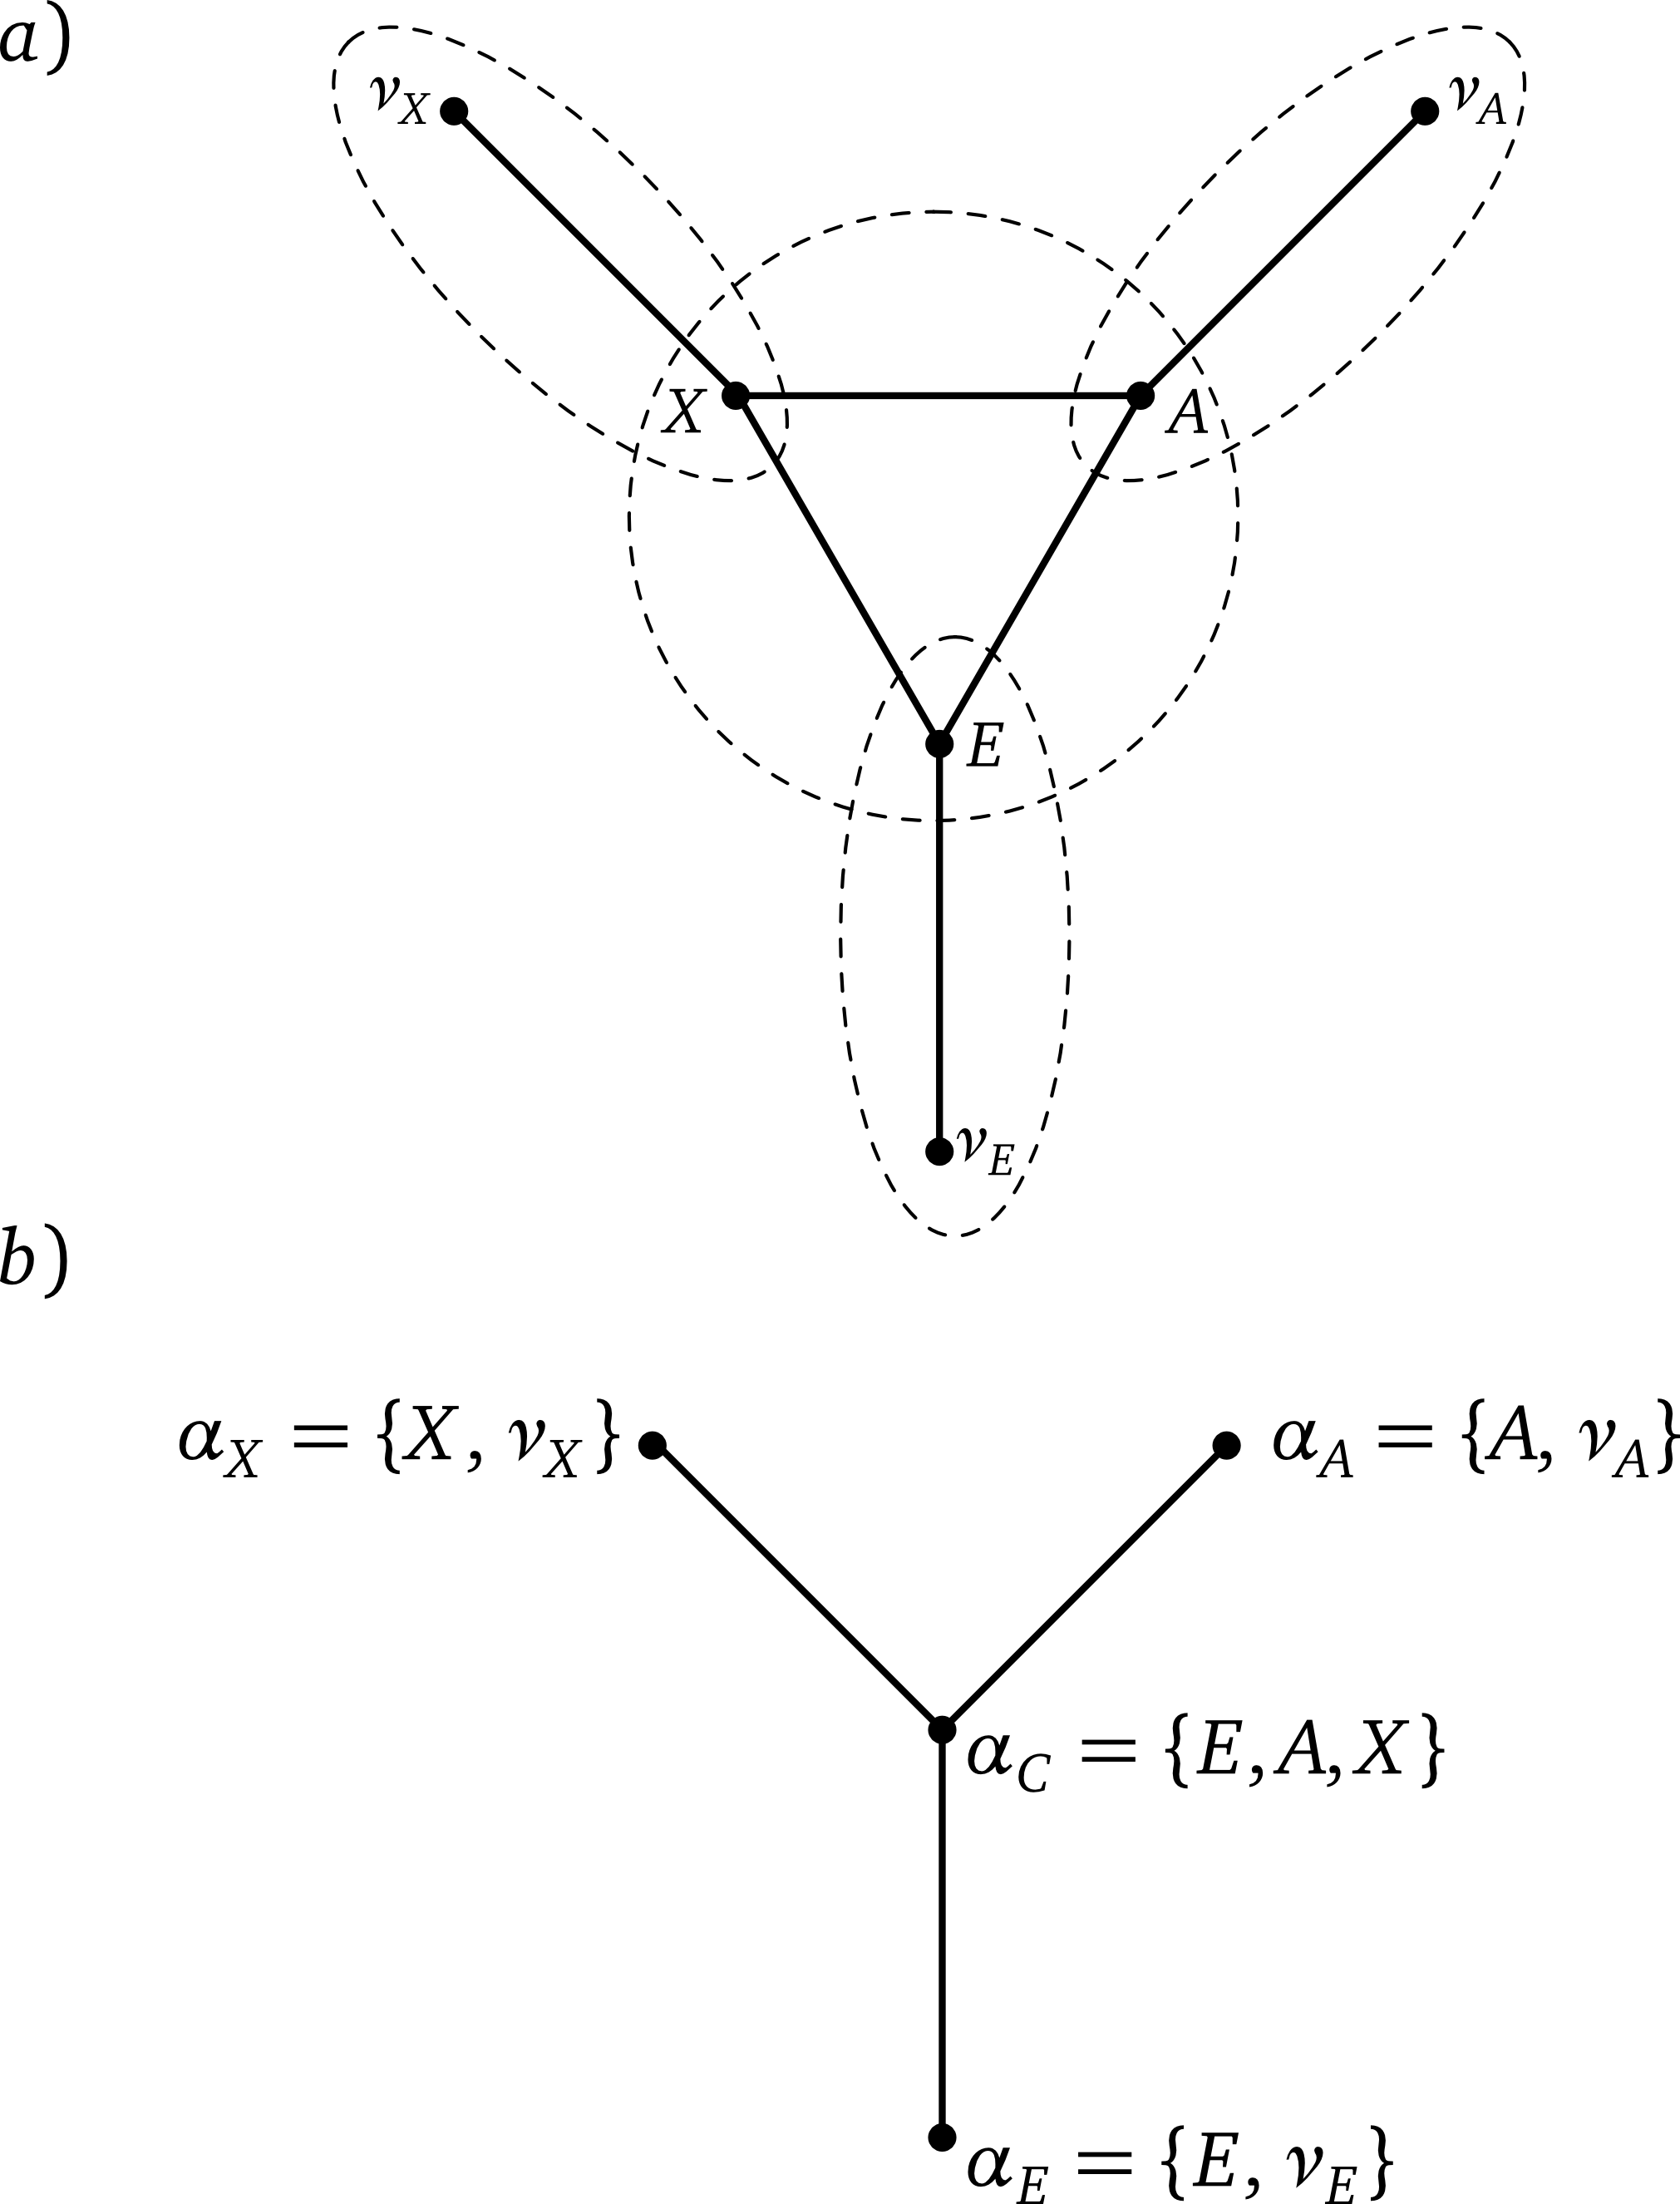
\includegraphics[width=10cm]{img/cliques.png}
  \end{center}
  \caption{a) The graph for the cross currency has four cliques. b) These cliques are the vertices of a new graph $\Gamma$. An edge in this new graph connects two cliques that have a non-empty intersection.}\label{fig.cliques}
\end{figure}

Because the graph $\gamma$ for the matrix $H$ is chordal, there exists a clique tree, i.e.  a spanning tree for the graph $\Gamma$ that possesses the intersection property. A spanning tree for $\Gamma$ is a tree that has the same vertices as the graph itself. It possesses the intersection property if for any two vertices $\alpha_1$ and $\alpha_2$ the intersection $\alpha_1\cap\alpha_2$ is contained in all the vertices on the unique path in the tree that connects $\alpha_1$ to $\alpha_2$ (see \cite{blair} for the different characterizations of a chordal graph). In our example the graph $\Gamma$ is itself a tree. It is also easy to check that it possesses the intersection property. In the next section we will see an example where the intersection property is not trivially fulfilled. We will choose $\alpha_E = \{E, \nu_E\}$ as the root of the tree. 

\begin{figure}[hbt]
  \begin{center}
  	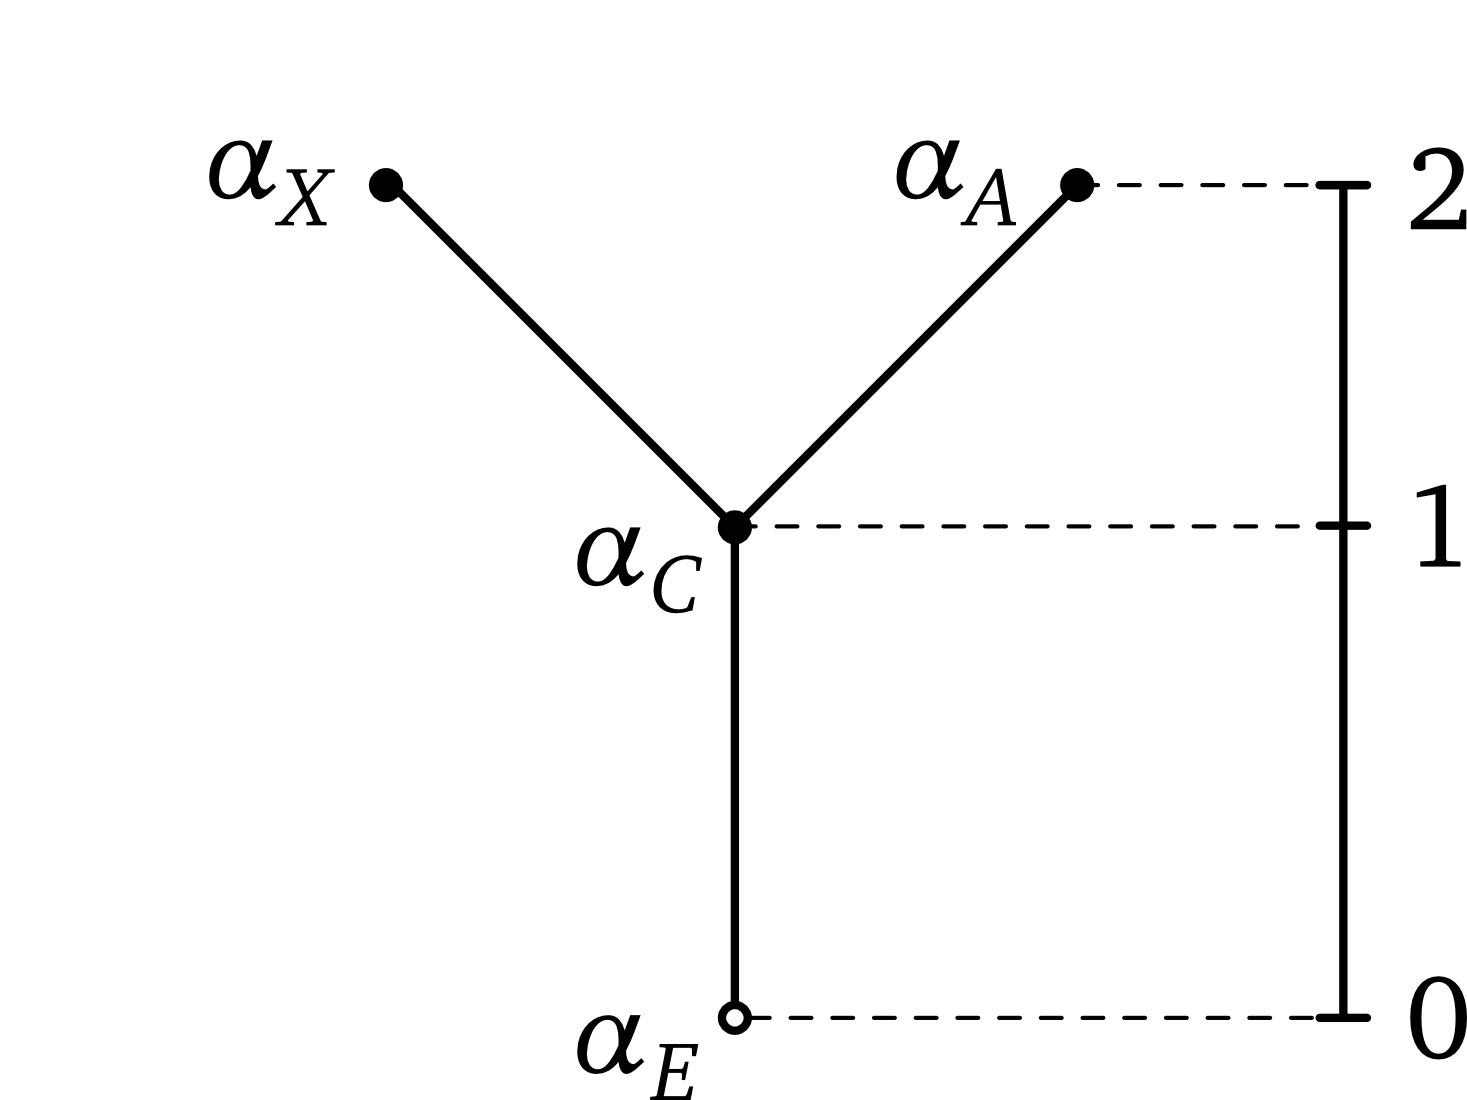
\includegraphics[width=10cm]{img/cliqueTree.png}
  \end{center}
  \caption{The clique tree for the graph $\gamma$. The numbers on the right denote the height in the tree if we choose $\alpha_E$ to be the root of the tree. The completion procedure proceeds from the top of the tree to the bottom. We complete the matrix by repeatedly using equation (\ref{eqn.choice}) from the previous section.}\label{fig.cliqueTree}
\end{figure}

We now start completing the matrix $H$ by repeatedly applying equation (\ref{eqn.choice}) from the previous section. We start with the cliques on the top of the tree and work our way down. We start with the clique $\alpha_X=\{X, \nu_X\}$. It intersects the clique $\alpha_C$ in the element $X$. This leads us to make the following identifications:
\begin{align}
	H_X & = \begin{pmatrix}
		1 & (X, \nu_X) \\
		& 1
	\end{pmatrix} \\
	H_Y & = \begin{pmatrix}
		1 & (E,X) & (A,X) \\
		& 1 & (E,A) \\
		& & 1 
	\end{pmatrix}
\end{align}
Note that the common matrix $C$ is just given by 1. Equation (\ref{eqn.choice}) now gives:
\begin{align}
	W & = ( (E,\nu_X), (A,\nu_X) ) \\
	& = BC^{-1}D \\
	& = (X, \nu_X) ( (E,X), (A,X) ) ) \\
	& =  ( (X, \nu_X)(E,X), (X, \nu_X)(A,X) ) ), 
\end{align}
or 
\begin{align}
	(E,\nu_X) & = (X, \nu_X)(E,X) \\
	(A,\nu_X) & = (X, \nu_X)(A,X).
\end{align}
Figure \ref{fig.firstStep} shows the first completion step in the graph $\gamma$. 

\begin{figure}[hbt]
  \begin{center}
  	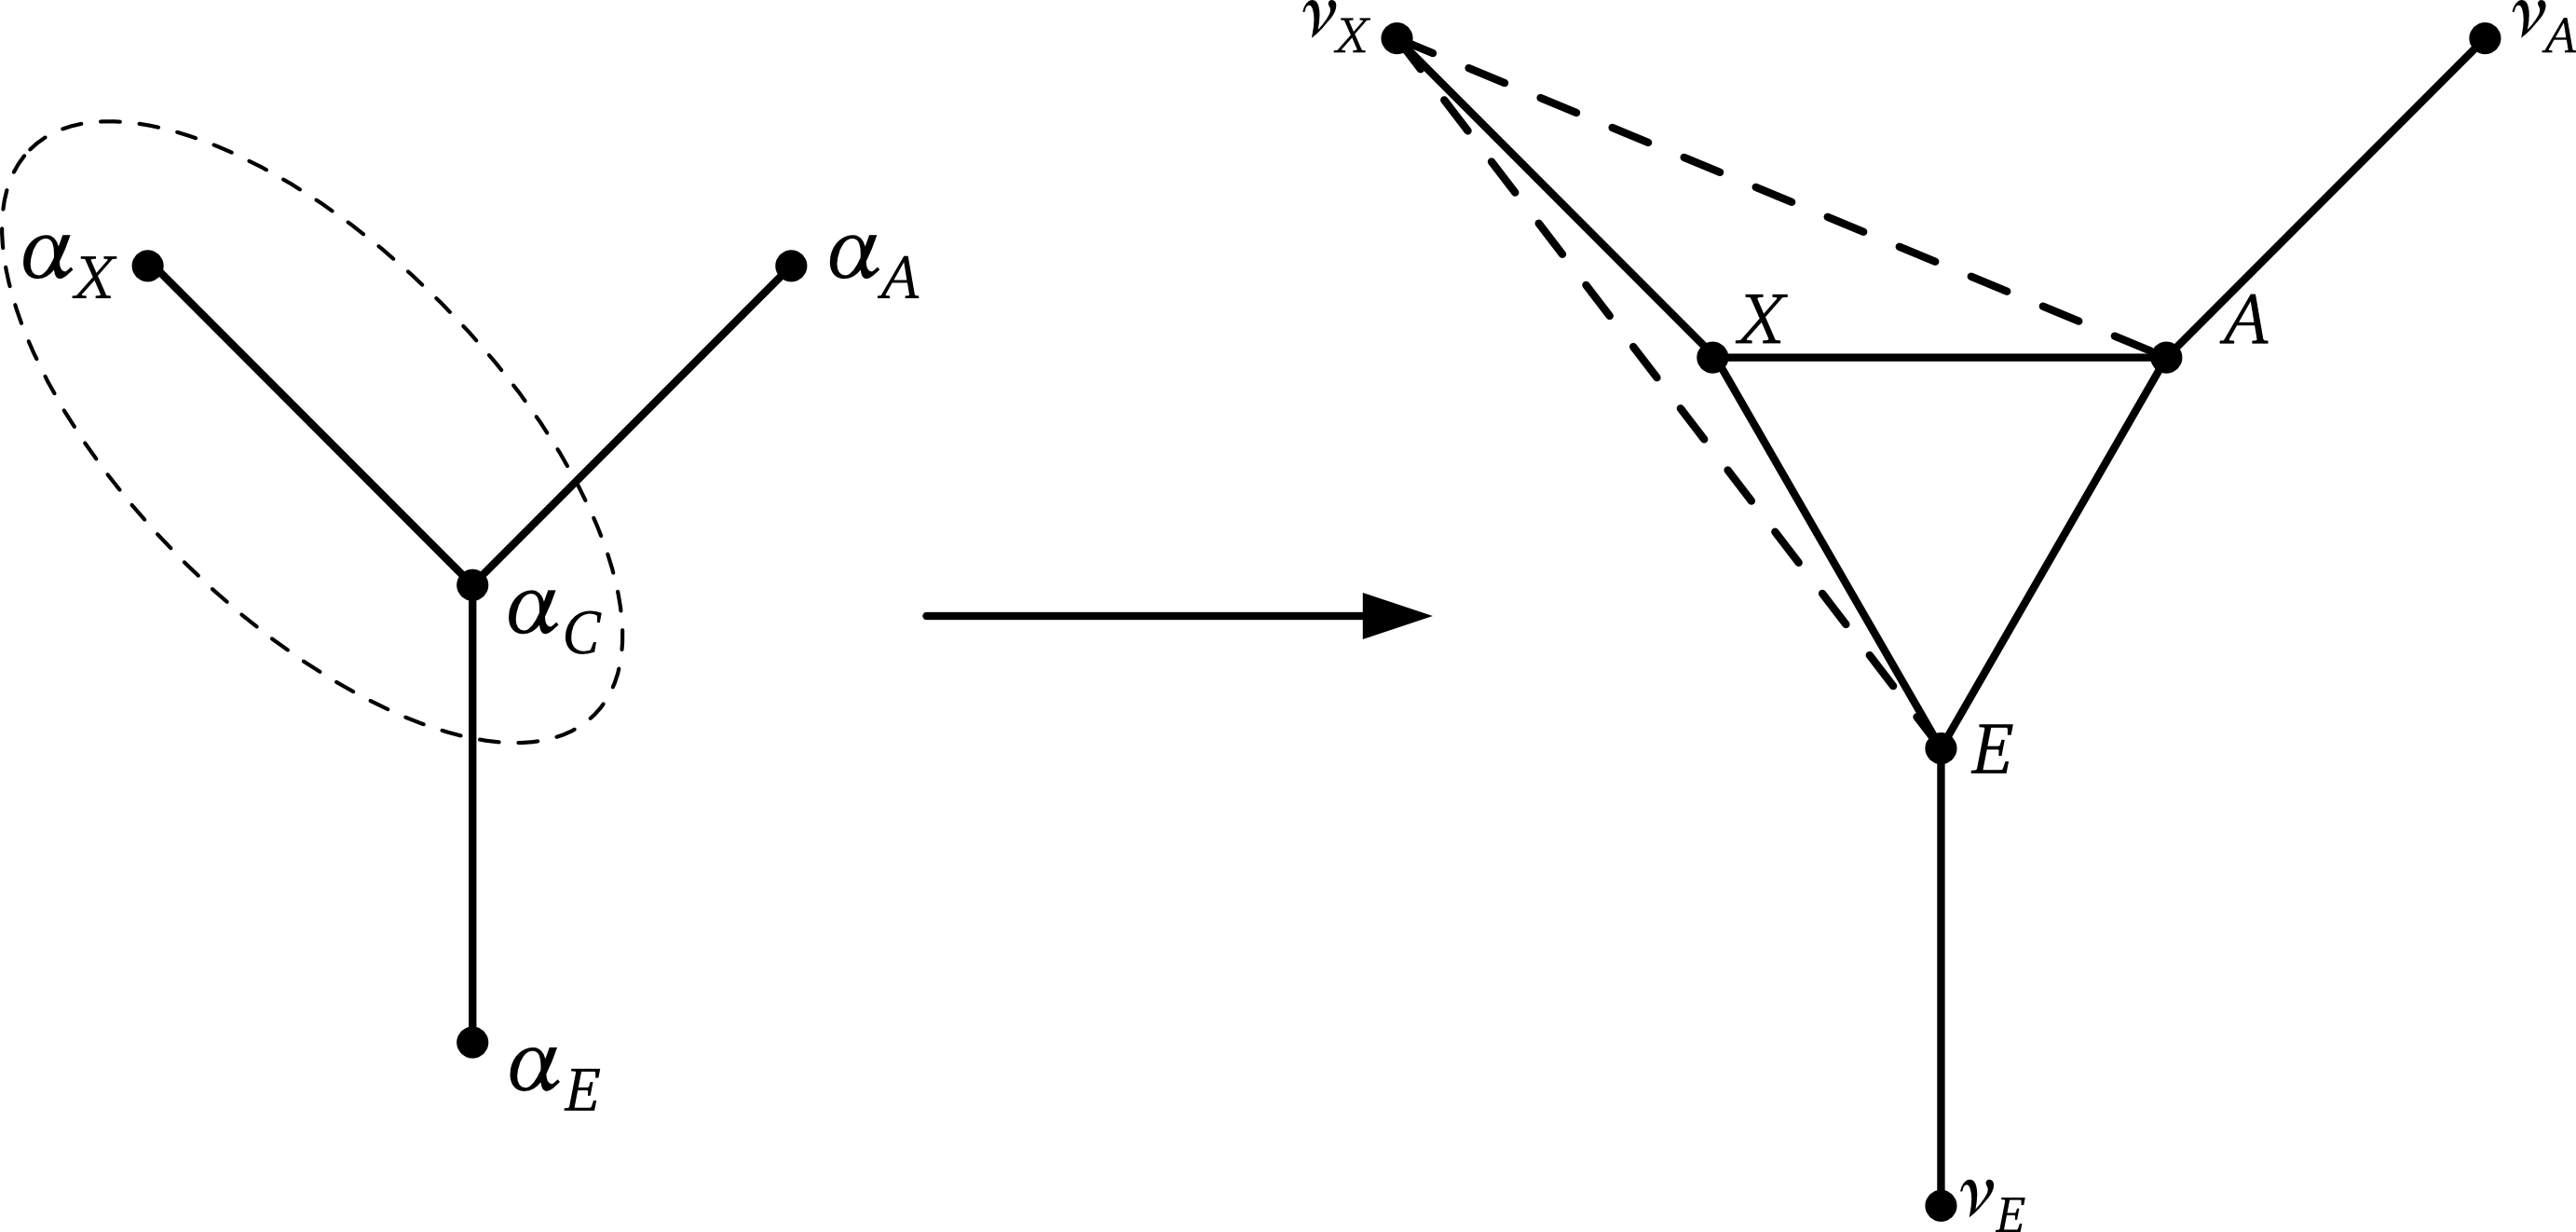
\includegraphics[width=10cm]{img/firstStep.png}
  \end{center}
  \caption{We start the completion of the matrix $H$ with the cliques of height two. Applying equation (\ref{eqn.choice}) to the matrices given by the cliques $\alpha_X$ and $\alpha_C$ adds the dashed lines to the graph $\gamma$.}\label{fig.firstStep}
\end{figure}

We have one more clique with height two in the clique tree for $\gamma$. In the next step we take the clique $\alpha_A$ and combine it with the newly created clique from the last step. This time we make the identifications
\begin{align}
	H_X & = \begin{pmatrix}
		1 & (A, \nu_A) \\
		& 1
	\end{pmatrix} \\
	H_Y & = \begin{pmatrix}
		1 & (A,E) & (A,X) & (A,\nu_X) \\
		& 1 & (E,X) & (E,\nu_X) \\
		& & 1 & (X,\nu_X) \\
		& & & 1 
	\end{pmatrix}
\end{align}
We apply equation (\ref{eqn.choice}) again to obtain:
\begin{align}
	W & = ( (E,\nu_A), (X,\nu_A), (\nu_X,\nu_A) ) \\
	& = BC^{-1}D \\
	& = (A,\nu_A) ( (E,A), (A,X), (A,\nu_X) ),
\end{align}
or
\begin{align}
	(E,\nu_A) & = (A,\nu_A) (E,A) \\
	(X,\nu_A) & = (A,\nu_A)(A,X)\\
	(\nu_X,\nu_A) & = (A,\nu_A) (A,\nu_X) \\
	& = (A,\nu_A)(X, \nu_X)(A,X)
\end{align}
Figure \ref{fig.secondStep} shows the result of this step in the graph $\gamma$. 

\begin{figure}[hbt]
  \begin{center}
  	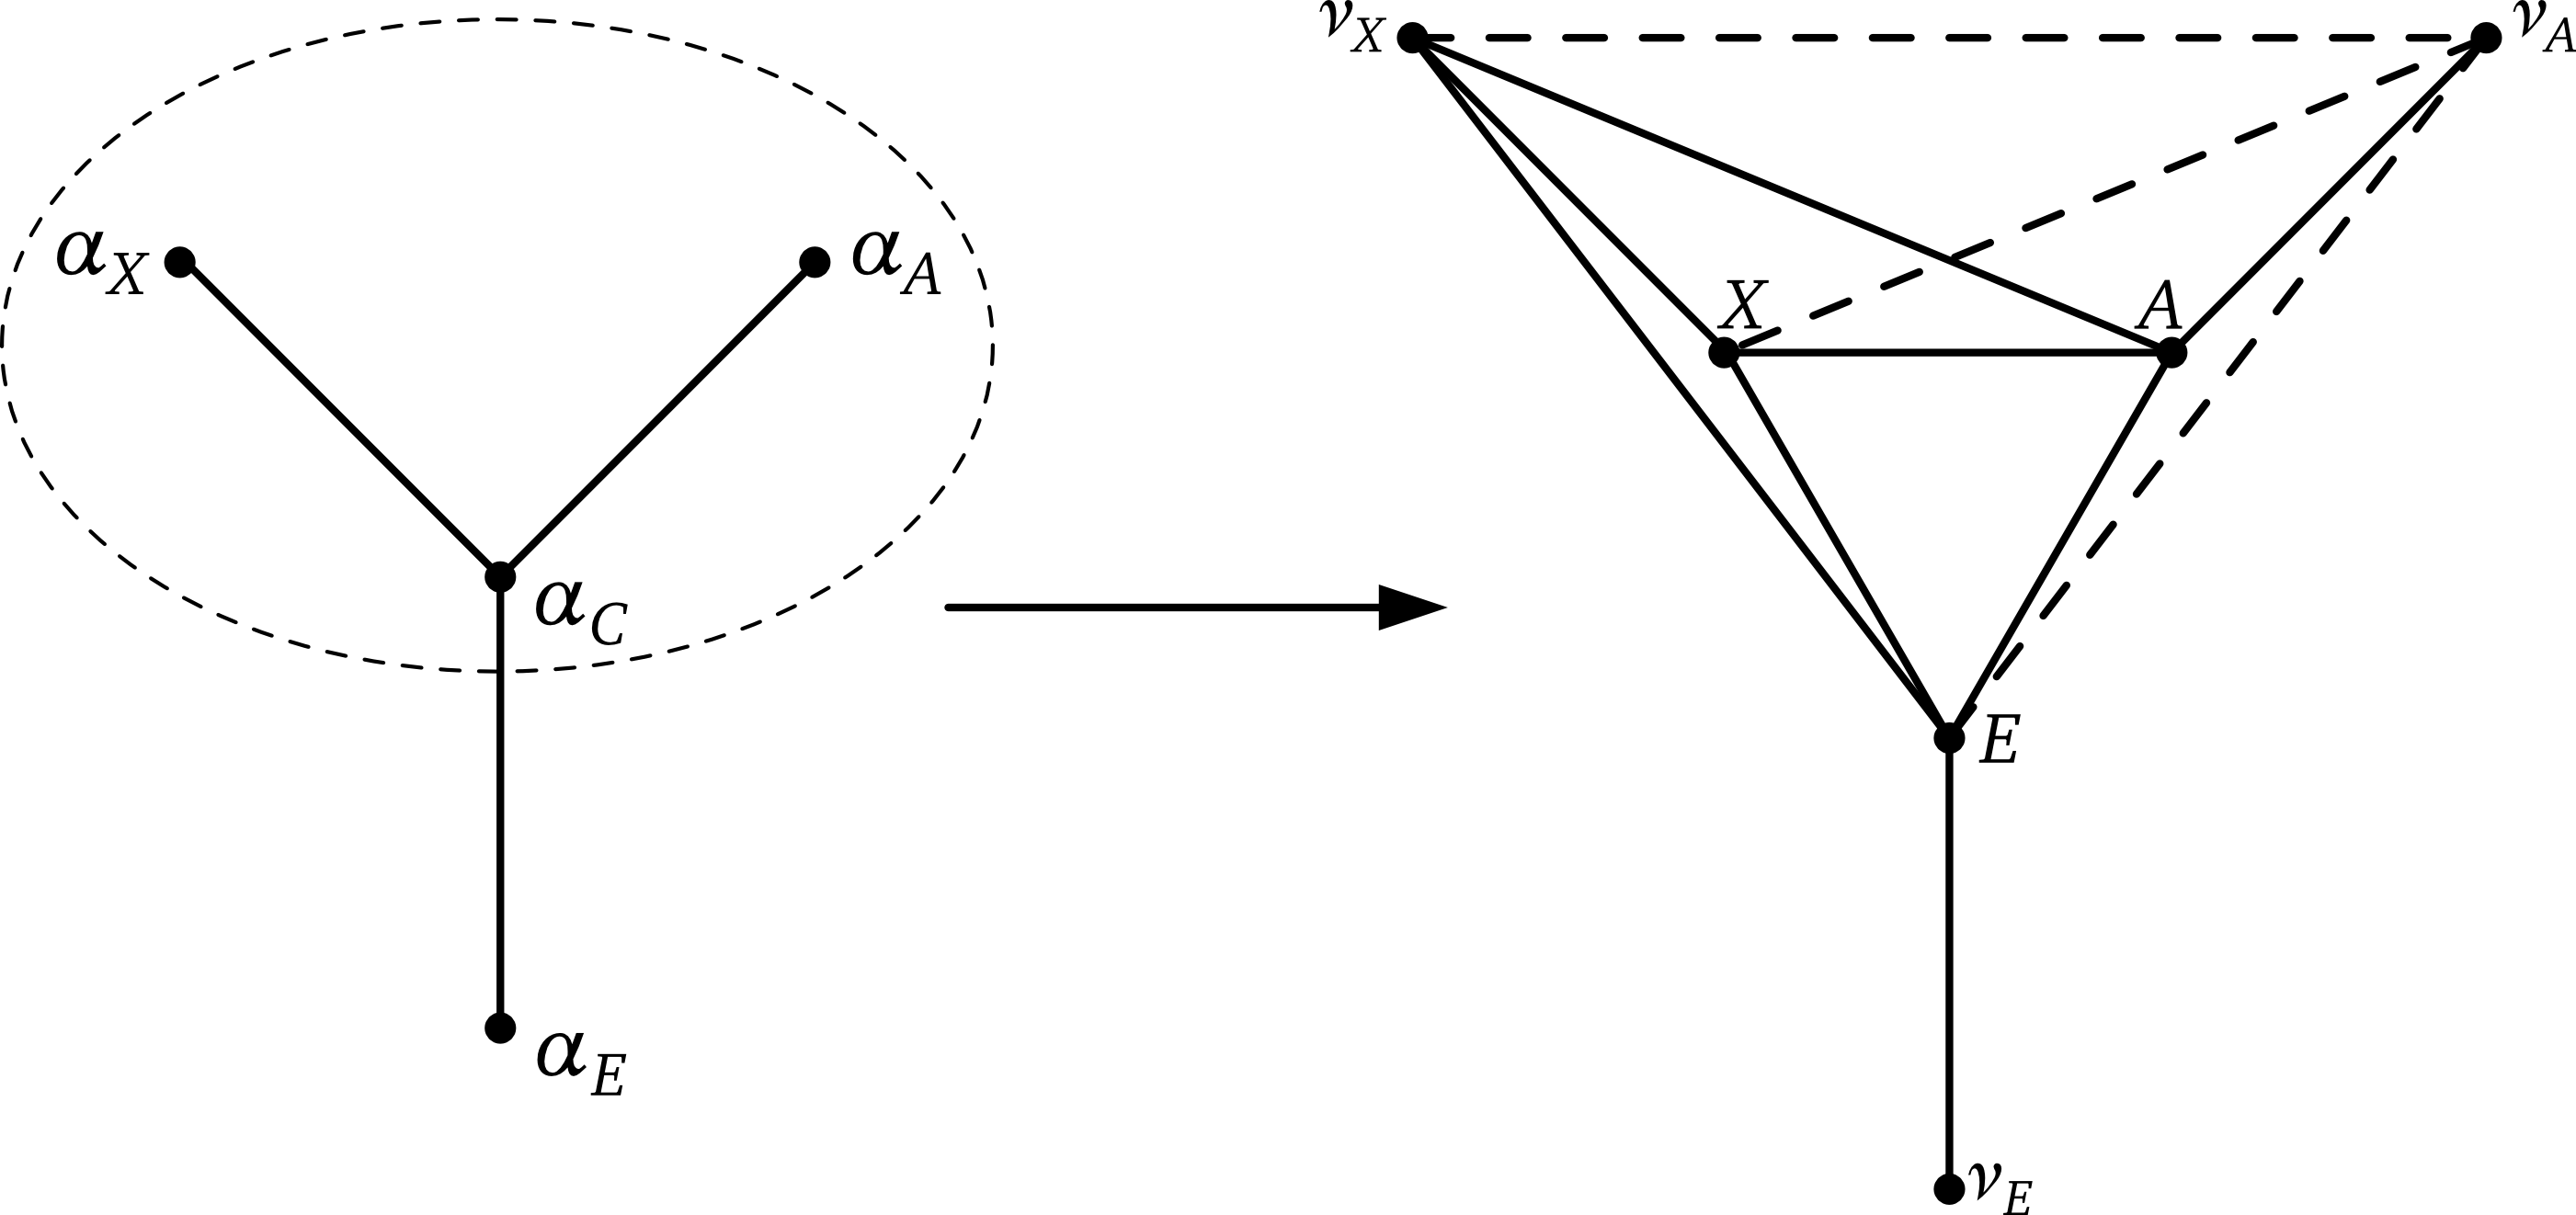
\includegraphics[width=10cm]{img/secondStep.png}
  \end{center}
  \caption{In the second step we combine the clique from the first step with the remaining clique of height two in the tree. This step adds the three edges $(\nu_X,\nu_A)$, $(X,\nu_A)$, and $(E,\nu_A)$.}\label{fig.secondStep}
\end{figure}

There are no more cliques of height two left. Looking at the graph in figure \ref{fig.secondStep} we see that only the edges connecting $\nu_E$ to the large clique that is the result of the last step are missing. These missing edges will be created in the last step. We make the following identifications:
\begin{align}
		H_X & = \begin{pmatrix}
		1 & (E, \nu_E) \\
		& 1
	\end{pmatrix} \\
	H_Y & = \begin{pmatrix}
		1 & (E,A) & (E,\nu_A) & (E,X) & (E,\nu_X) \\
		& 1 &  (A,\nu_A) & (A,X) & (A,\nu_X) \\
		& & 1 & (\nu_A,X) & (\nu_A,\nu_X) \\
		& & & 1 & (X,\nu_X) \\
		& & & & 1 
	\end{pmatrix}
\end{align}
Applying equation (\ref{eqn.choice}) one more time gives:
\begin{align}
	W &= ( (\nu_E,A),(\nu_E,\nu_A),(\nu_E,X),(\nu_E,\nu_X) ) \\ 
	& = BC^{-1}D \\
	& = (E, \nu_E) ( (E,A),(E,\nu_A),(E,X),(E,\nu_X) ), 
\end{align}
or
\begin{align}
	(\nu_E,A) & = (E, \nu_E) (E,A) \\
	(\nu_E,\nu_A) & = (E, \nu_E) (E,\nu_A) \\
	& = (E, \nu_E) (A,\nu_A) (E,A) \\
	(\nu_E,X) & = (E, \nu_E) (E,X) \\
	(\nu_E,\nu_X) & = (E, \nu_E) (E,\nu_X) \\
	& = (E, \nu_E) (X, \nu_X)(E,X)
\end{align}
With this step we have added the last missing edges in the graph $\gamma$ and have obtained a positive definite completion of the matrix $H$.

\section{Several currencies}
In the previous section we have just looked at one foreign currency $A$ with one exchange rate $X$. The procedure can easily be extended to an arbitrary number of foreign currencies. We will denote the foreign currencies by a capital letter:
\begin{equation}
	A, B, C, \ldots
\end{equation}
The exchange rate between the domestic currency $E$ and the foreign currency $A$ will now be denoted by 
\begin{equation}
	X_E^A.
\end{equation}
If $m_A$ is an amount in currency $A$ then $X_E^Am_A$ is the corresponding amount in currency $E$. If we are given the same correlation coefficients as in the previous section we obtain the graph in figure \ref{fig.several}. The corresponding graph of cliques is shown in figure \ref{fig.severalCliques}. The corresponding clique tree is obtained by erasing the lines that connect the cliques 
\begin{equation}
	\alpha_{CA}, \alpha_{CB}, \ldots, \alpha_{CG}
\end{equation}
on the middle layer. The intersection of any two of these cliques is given by
\begin{equation}
	\{E\} \subset \alpha_E.
\end{equation}
Since the path connecting the two cliques passes through $\alpha_E$ this tree satisfies the intersection property. 

\begin{figure}[hbt]
  \begin{center}
  	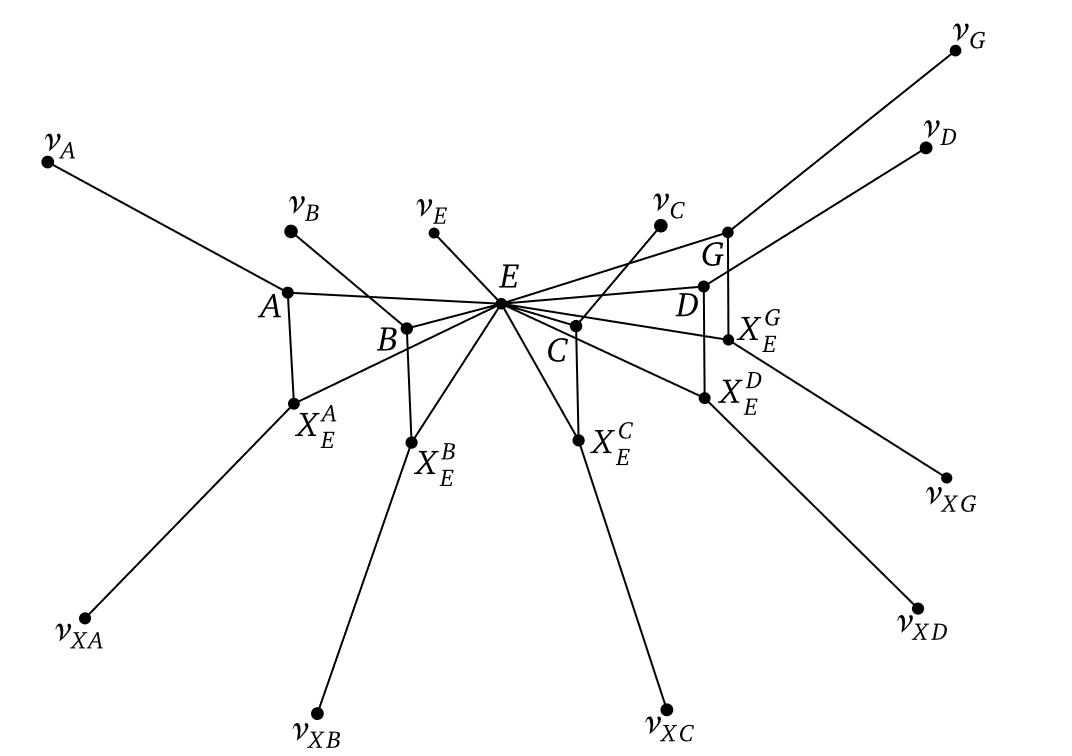
\includegraphics[width=10cm]{img/severalCurrencies.png}
  \end{center}
  \caption{The graph corresponding to the incomplete correlation matrix for five foreign currencies.}\label{fig.several}
\end{figure}

\begin{figure}[hbt]
  \begin{center}
  	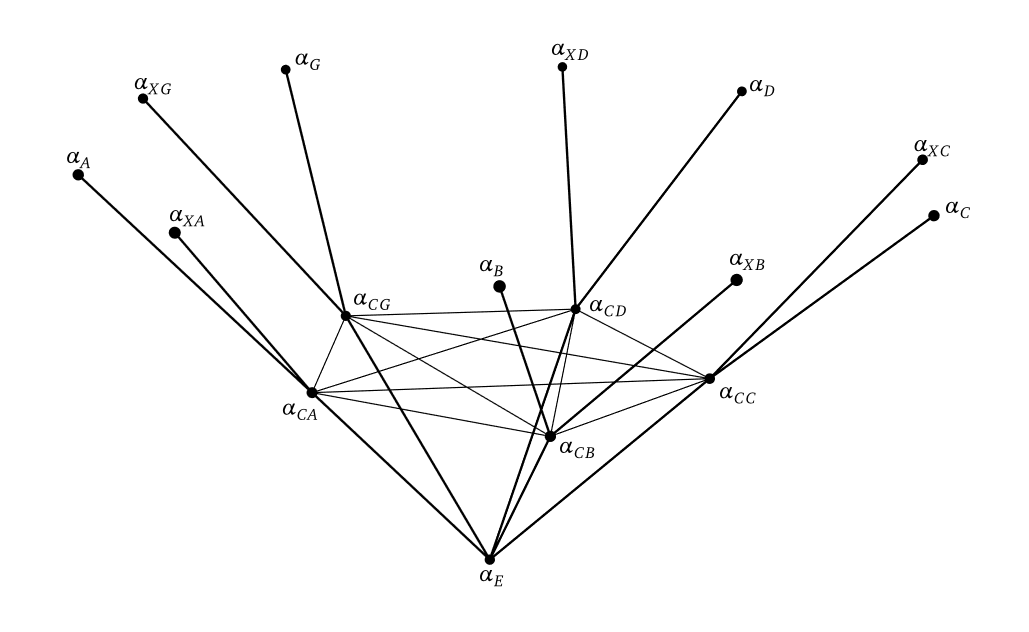
\includegraphics[width=12cm]{img/severalCurrCliques.png}
  \end{center}
  \caption{The graph of cliques for the case of several foreign currencies. A clique tree is obtained by removing the lighter edges in the middle layer. It is again a tree of height two.}\label{fig.several}
\end{figure}




\section{Conclusion}

\begin{thebibliography}{MM}
	\bibitem{rao} C. Radharkishna Rao, Linear Statistical Inference and its Applications, 2nd edition, John Wiley \& Sons, Inc, 2002.
	\bibitem{cottle} Richard W. Cottle, Manifestations of the Schur complement, Linear Algebra and its Applications \textbf{8}, 1974, 189--211. 
	\bibitem{hayns} Emilie Virginia Haynsworth, Determination of the inertia of a partitioned Hermitian matrix,  Linear  Algebra and its Applications \textbf{1}, 1968, 73--81.
	\bibitem{schur} J. Schur, �ber Potenzreihen, die im Innern des Einheitskreises beschr�nkt sind, Journal f�r die reine und angewandte Mathematik \textbf{147}, 205 -- 232, 1917.
	\bibitem{horn} Roger A. Horn, Basic  Properties  of  the  Schur  Complement. In Fuzhen Zhang (Ed.) The Schur complement and its application (17--46). Springer, 2005.
	\bibitem{grone} R. Grone, C.R. Johnson, E. Sa, H. Wolkowicz, Positive definite completion of partial Hermitian matrices, Linear Algebra Appl. 58, 109--124, 1984.
	\bibitem{smith} R. L. Smith, The positive definite completion problem revisited, Linear Algebra and its Applications 429 (2008) 1442 -- 1452.
	\bibitem{ksd} our other paper ...
	\bibitem{golumbic} M. C. Golumbic, Algorithmic Graph Theory and Perfect Graphs, Elsevier, 2004. 
	\bibitem{blair} Jean R. S. Blair, Barry Peyton, An introduction to chordal graphs and clique trees, in Alan George, John R. Gilbert, Joseph W. H. Liu (Eds.), Graph Theory and Sparse Matrix Computation (pp. 1 -- 29), The IMA Volumes in Mathematics and its Applications, 56, Springer Verlag, 1993.
\end{thebibliography}

\end{document}